\documentclass[useAMS,usenatbib]{mn2e}
%\documentclass[twocolumn]{emulateapj}
\usepackage{graphicx,natbib,color,multirow,amsmath}
\voffset=-0.8in

\definecolor{titlecol}{rgb}{0,0,1}
\definecolor{titlecol2}{rgb}{0,0.65,0}
\definecolor{titlecol3}{rgb}{0.99,0.4,0.}

%\definecolor{titledark}{rgb}{0,0,0.8}
%\definecolor{hilit}{rgb}{0,0,1}
%\definecolor{hilitdark}{rgb}{0,0,0.8}
%\font\sbf=cmssbx10 at 32.28pt %big font for headers

\font\nbf=cmssbx10 at 12.28pt %big font for headers

%%%%%%%%%%%%%%%%%%%%%%%%%%%%%%%
%%%% If you want to leave notes in the text feel free to define
%%%% your own colour above and a style below
%%%%%%%%%%%%%%%%%%%%%%%%%%%%%%%
\def\note		{\color{titlecol2} \nbf}
\def\noteb		{\color{titlecol} \nbf}
\def\notebsm	{\color{titlecol}}
\def\notec		{\color{titlecol2} \nbf}
\def\notecsm	{\color{titlecol2}}
\def\notek		{\color{titlecol3} }
\def\builderUC       {} % builder, unconfirmed

%%%%%%%%%%%%%%%%%%%%%%%%%%%%%%%
% For the eventual referee response
\def\changed    {\color{titlecol} }
%\def\changed    {}


%%%%%%%%%%%%%%%%%%%%%%%%%%%%%%%
%  Other stuff I use a lot
\def\oiii		{$\mathrm{\left[ O \textsc{iii}\right] }$}
\def\moiii		{\mathrm{\left[ O \textsc{iii}\right] }}
\def\nii		{$\mathrm{\left[ N \textsc{ii}\right] }$}
\def\mnii		{\mathrm{\left[ N \textsc{ii}\right] }}
\def\sii		{$\mathrm{\left[ S \textsc{ii}\right] }$}
\def\msii		{\mathrm{\left[ S \textsc{ii}\right] }}
\def\galfit     {{\tt GALFIT}}

\def\mmsun	{\rm{M}_{\odot}}
\def\fnobulge    {$f_{\rm no~bulge}$}
\def\mfnobulge {f_{\rm no~bulge}}
\def\fedgeon     {$f_{\rm edge-on}$}
\def\mfedgeon  {f_{\rm edge-on}}
\def\fcnobulge    {$f_{\rm confirmed~no~bulge}$}
\def\mfcnobulge {f_{\rm confirmed~no~bulge}}

\def\kappamean {$\overline{\kappa}$}
\def\mkappamean {\overline{\kappa}}


%\def\lesssim{\mathrel{\hbox{\rlap{\hbox{\lower5pt\hbox{$\sim$}}}\hbox{$<$}}}}
%\def\gtrsim{\mathrel{\hbox{\rlap{\hbox{\lower5pt\hbox{$\sim$}}}\hbox{$>$}}}}
%new defs of lesssim gtrsim that I think look better
\def\lesssim{\mathrel{\hbox{\rlap{\hbox{\lower3pt\hbox{$\sim$}}}\hbox{\raise2pt\hbox{$<$}}}}}
\def\gtrsim{\mathrel{\hbox{\rlap{\hbox{\lower3pt\hbox{$\sim$}}}\hbox{\raise2pt\hbox{$>$}}}}}


\newcommand\nodata{ ~$\cdots$~ }




\begin{document}

\title[Galaxy Zoo: CANDELS Data Release]{Galaxy Zoo: Detailed Morphological Classifications for 48,000 galaxies from CANDELS\thanks{This publication has been made possible by the participation of more than 95,000 volunteers in the Galaxy Zoo project. The contributions of the more than $40,000$ of those who registered a username with Galaxy Zoo are
individually acknowledged at http://authors.galaxyzoo.org/ .} } 

\author[Simmons et al.]{\parbox[t]{16cm}{B. D. Simmons$^{1}\thanks{E-mail: brooke.simmons@astro.ox.ac.uk}$, {\notebsm and a \emph{lot} of other people to be named later}
%Chris Lintott$^{1,3}$, 
%Kyle W. Willett$^{5}$, 
%Karen L. Masters$^{2,4}$, 
%Robert C. Nichol$^{2,4}$, 
%William C. Keel$^{6}$, 
%Thomas Melvin$^{2}$, 
%R. J. Smethurst$^{1}$, 
%Edmond Cheung$^{7}$, 
%Kevin Schawinski$^{8}$, 
%Michael Rutkowski$^{5}$,
%Jeyhan S. Kartaltepe$^{9,}$\footnote{Hubble Fellow}, 
%Kevin R. V. Casteels$^{11}$, 
%Christopher J. Conselice$^{12}$,
%Omar Almaini$^{12}$, 
%Henry C. Ferguson$^{13}$,
%Lucy Fortson$^{5}$, 
%William Hartley$^{12,8}$, 
%Dale Kocevski$^{14}$,
%Anton M. Koekemoer$^{13}$,
%Daniel H. McIntosh$^{15}$,
%Alice Mortlock$^{12}$, 
%{\builderUC Jeffrey A. Newman$^{16}$,}
%Jamie Ownsworth$^{12}$, 
%Steven Bamford$^{12}$,
%{\builderUC Tomas Dahlen$^{13}$,} 
%{\builderUC Sandra M. Faber$^{17}$,}
%{\builderUC Steven L. Finkelstein$^{18}$,} 
%{\builderUC Adriano Fontana$^{19}$,}
%{\builderUC Audrey Galametz$^{19}$,}
%N. A. Grogin$^{13}$,
%{\builderUC Ruth Gr\"utzbauch$^{12, 20}$,} 
%{\builderUC Yicheng Guo$^{17}$,}
%{\builderUC Boris H\"au\ss ler$^{12,21,1}$,}
%Kian Jek$^{22}$,
%Sugata Kaviraj$^{21}$,
%Ray A. Lucas$^{13}$,
%{\builderUC Michael Peth$^{23}$,}
%{\builderUC Mara Salvato$^{24}$,} 
%{\builderUC Tommy Wiklind$^{25}$,} 
%{\builderUC Stijn Wuyts$^{24}$}
%
\vspace{0.1in} }\\
$^{1}$Oxford Astrophysics, Denys Wilkinson Building, Keble Road, Oxford OX1 3RH, UK\\
%$^{2}$Institute of Cosmology \& Gravitation, University of Portsmouth, Dennis Sciama Building, Portsmouth PO1 3FX, UK\\
%$^{3}$Adler Planetarium, 1300 S. Lake Shore Drive, Chicago, IL 60605, USA\\
%$^{4}$SEPnet,\thanks{www.sepnet.ac.uk} South East Physics Network\\
%$^{5}$School of Physics and Astronomy, University of Minnesota, 116 Church St. SE, Minneapolis, MN 55455, USA\\
%$^{6}$Department of Physics and Astronomy, University of Alabama, Box 870324, Tuscaloosa, AL 35487, USA\\
%$^{7}$Department of Astronomy and Astrophysics, 1156 High Street, University of California, Santa Cruz, CA 95064, USA\\
%$^{8}$Institute for Astronomy, ETH Z\"urich, Wolfgang-Pauli-Strasse 27, CH-8093 Z\"urich, Switzerland\\
%$^{9}$National Optical Astronomy Observatory, 950 N. Cherry Ave., Tucson, AZ, 85719, USA\\
%$^{10}$Department of Astronomy, University of Michigan, Ann Arbor, MI 48104, USA\\
%$^{11}$Institut de Cincies del Cosmos. Universitat de Barcelona (UB-IEEC), Mart i Franqus 1, E-08028 Barcelona, Spain\\
%$^{12}$School of Physics \& Astronomy, University of Nottingham, Nottingham NG7 2RD\\
%$^{13}$Space Telescope Science Institute, 3700 San Martin Drive, Baltimore, MD 21218\\
%$^{14}$Department of Physics and Astronomy, University of Kentucky, Lexington, KY 40506, USA\\
%$^{15}$Department of Physics, University of Missouri-Kansas City, 5110 Rockhill Road, Kansas City, MO 64110, USA\\
%$^{16}$Department of Physics and Astronomy \& PITT PACC, University of Pittsburgh, Pittsburgh, PA 15217, USA\\
%$^{17}$UC Observatories/Lick Observatory and Department of Astronomy and Astrophysics, University of California, Santa Cruz, CA 95064, USA\\
%$^{18}$Department of Astronomy, The University of Texas at Austin, Austin, TX 78712, USA\\
%$^{19}$INAF-Osservatorio Astronomico di Roma, Via Frascati 33, I-00040, Monteporzio, Italy\\
%$^{20}$Centre for Astronomy and Astrophysics, University of Lisbon, P-1349-018 Lisbon, Portugal\\
%$^{21}$Centre for Astrophysics Research, University of Hertfordshire, College Lane, Hatfield AL10 9AB, UK\\
%$^{22}$Galaxy Zoo Volunteer\\
%$^{23}$Department of Physics and Astronomy, The Johns Hopkins University, Baltimore, MD 21218, USA\\
%$^{24}$Max-Planck-Institut f{\"u}r extraterrestrische Physik, Giessenbachstrasse 1, D�85748 Garching bei M{\"u}nchen, Germany\\
%$^{25}$European Southern Observatory/Joint ALMA Observatory, 3107 Alonso de Cordova, Santiago, Chile\\
   }

\maketitle
  
\label{firstpage}
  
%\clearpage

\begin{abstract}

{\notebsm To be rewritten, probably last.}

Galaxies are sometimes really far away. The distant ones are pretty cool, because they tell us what the Universe was like back when it was just a kid, or maybe a teenager. You really have to look hard to see these galaxies, but once you do, what you do see tells you a whole lot. I mean, it's not exactly a WYSIWYG type of thing: there's a lot of work to figure out what the faint stuff you see really means. We did a bunch of work, and we think we did pretty well. Also, we compared to others who have done different kinds of work to try and answer some of the same questions. But we have a unique way of answering them, so here are those answers, and you can use them to answer other questions about the Universe.


  \end{abstract}
  
  \begin{keywords}
  
  galaxies: general 
  --- 
  galaxies: evolution
  --- 
  galaxies: morphology %not actually a keyword 
  --- 
  galaxies: structure
  
  \end{keywords}

%%%%%%%%%%%%%%%%%%%%%%%%%%%%%%%%%%%%%%%%%%%%%%
%
%  
\section{Introduction}
%
%
%%%%%%%%%%%%%%%%%%%%%%%%%%%%%%%%%%%%%%%%%%%%%%

This paper presents morphological classifications of nearly $50,000$ galaxies imaged in the Cosmic And Near-infrared Deep Extragalactic Legacy Survey \citep[CANDELS;][]{grogin11,koekemoer11} measured by the Galaxy Zoo{\footnote{zoo4.galaxyzoo.org}} project \citep{lintott08}. Over 95,000 volunteers have contributed over 2,000,000 detailed galaxy classifications to this effort. We combine, on average, 43 independent classifications of each galaxy to produce detailed, quantitative morphological descriptions of these distant galaxies along many physical axes of interest. 

% for each of the morphology citation bombs below it would be good to have some non-GZ papers in there.
The shape and appearance of a galaxy trace the underlying physical processes that have formed it and continue to influence its evolution. For example, the signatures of past merger events \citep[from $z \sim 2$ onwards;][]{martig12} are visible even at $z = 0$ in the form of a galactic bulge; the strength of the bulge is tied to the strength of the merger, as indeed the lack of a bulge indicates a lack of significant mergers \citep[e.g.,][]{kormendy10}. Likewise, other morphological features are tied to disk instabilities and resonances \citep[e.g., warps, bars, rings][]{dunno, dunno}, and orbital changes from the disruptive \citep[mergers; e.g.,][]{darg10a,darg10b,lotz_unsureofyear,others} to the relatively subtle \citep[e.g., bars,][]{sometheorypapershere,wouldbegood}. Furthermore, combination of morphological parameters with other measures, such as environment, color, mass and star formation histories \citep[e.g.][]{bamford09,tojiero_yearpls,schawinski14,smethurst15}, can provide more insight than either alone.

Morphological measures have a long history in astronomy \citep[e.g.,][]{hubble26,a,few,more,pls}. The computerized era of astrophysics has brought with it a number of automated morphological classification techniques. Some use multiple parameters to characterise a galaxy's distribution of light \citep{sersic68,oneofthefouriermodepapers,etc}, while others adopt a non-parametric approach, each reducing a galaxy to one number \citep[and often used in combination; e.g.][]{gini,m20,abrahamCA,conseliceCAS,zestmaybe}. These lend themselves relatively well to large-scale processing of images from galaxy surveys \citep[e.g.][]{simard,griffith,lackner,zest} and provide a uniform quantitative set of measures. Modern machine learning techniques are also well-tested and applicable to large data sets \citep{huertascompany,kagglepaperifwecan}.

However, no computer has yet exceeded the human brain's capacity for pattern detection and serendipitous discovery. Visual morphologies remain among the most nuanced and powerful measures of galaxy structure. Galaxy Zoo combines the strengths of both visual and computer-driven approaches, using the Internet to collect more independent and complete visual classifications than any group of astronomers is realistically capable of and combining these classifications via tested and proven techniques.

Since 2007, Galaxy Zoo has been a unique resource of quantitative and statistically robust visual galaxy morphologies. Prior to Galaxy Zoo CANDELS, three Galaxy Zoo projects have collected morphologies for over $1,000,000$ galaxies using the largest surveys to date to $z \sim 1$. These projects have been and continue to be extremely scientifically productive, both for the project team \citep{citation,love,come,on,group,hug} and for the larger scientific community \citep{because,that,self,cite,thing,just,now,was,alittlecheeky}.

Here we present the Galaxy Zoo visual morphologies of $49,555$ galaxies imaged by the largest near-infrared \emph{Hubble Space Telescope (HST)} survey to date, CANDELS, which images galaxies at rest-frame optical wavelengths to $z \approx 2.7$. 

In Section \ref{sec:data} we describe the observational data and the preparation of CANDELS images for use in Galaxy Zoo. In Section \ref{sec:classifications} we detail the collection of morphological classifications and the method of weighting and combining independent classifications for each galaxy. Section \ref{sec:comparison} compares Galaxy Zoo classifications to other morphological measurements. In Section \ref{sec:result} we show an example result using the classifications, and in Section \ref{sec:summary} we summarize. Throughout
this paper we use the AB magnitude system, and where necessary we adopt a cosmology consistent with $\Lambda$CDM, with $H_{\rm 0}=70~{\rm
km~s^{-1}}$Mpc$^{\rm -1}$, $\Omega_{\rm m}=0.3$ and $\Omega_{\rm \Lambda}=0.7$ \citep{bennett13}.




%%%%%%%%%%%%%%%%%%%%%%%%%%%%%%%%%%%%%%%%%%%%%%
%
%
\section{Observational Data}\label{sec:data}
%
%
%%%%%%%%%%%%%%%%%%%%%%%%%%%%%%%%%%%%%%%%%%%%%%

\subsection{Images}\label{sec:images}

% Note this paragraph is lifted directly from the bar paper so I should probably mix it up a bit later
The Cosmic Assembly Near-infrared Extragalactic Legacy Survey \citep[CANDELS;][]{grogin11,koekemoer11} is an \emph{HST} Treasury programme combining optical and near-infrared imaging from the Advanced Camera for Surveys (ACS) and Wide Field Camera 3 (infrared channel; WFC3/IR) across five well-studied survey fields {(GOODS-North and -South, \citeauthor{giavalisco04} \citeyear{giavalisco04}; EGS, \citeauthor{davis07} \citeyear{davis07}; UDS, \citeauthor{lawrence07} \citeyear{lawrence07}, \citeauthor{cirasuolo07} \citeyear{cirasuolo07}; and COSMOS, \citeauthor{scoville07} \citeyear{scoville07}) using a two-tiered ``deep'' and ``wide'' approach. Each of the wide fields (UDS, COSMOS, EGS and flanking fields to the GOODS-S and GOODS-N deep fields) are imaged over 2 orbits in WFC3/IR, split in a 2:1 ratio between filters F160W and F125W, respectively, with parallel exposures in F606W and F814W using ACS. Each of the deep fields (GOODS-S and GOODS-N) are imaged over at least 4 orbits each in both the F160W and F125W filters and 3 orbits in the F105W filter, with ACS exposures in F606W and F814W in parallel. These are reduced and combined to produce a single mosaic for each field in each band, with drizzled resolutions of $0.03^{\prime\prime}$ and $0.06^{\prime\prime}$ per pixel for ACS and WFC3/IR, respectively \citep[a process described in detail by][]{koekemoer11}.

Here we use the CANDELS ACS and WFC3/IR images from within the first set of data to be classified within the Galaxy Zoo interface. Those data cover the COSMOS, GOODS-South, and UDS fields. The 4th release of Galaxy Zoo included all detections with $H \leq 25.5$ from these 3 combined fields, comprising 49,555 unique images. These were shown to visitors to the website galaxyzoo.org starting on the 10th of September, 2012.  

The images shown to the public are colour composites of ACS $I$ ($F814W$), WFC3 $J$ ($F125W$), and WFC3 $H$ ($F160W$) filters for the blue, green and red channels, respectively. The angular sizes of the images in different filters are matched, and the native point-spread functions (PSFs) are used. The images are combined with an asinh stretch \citep[described in detail in][]{luptonasinh} with a non-linearity value of {\notebsm 3.0}. 

Sources in the dataset vary greatly in size and surface brightness, and therefore a single set of values for channel scalings is not adequate to capture the variety of features across the images. We therefore use a variable scaling based on the {\notebsm magnitude and size} of each target source. For each image the R, G, and B channels have a fixed ratio of {\notebsm [not sure; must get this from Jeyhan]}, and the multiplier can vary between {\notebsm A and B}. Figure \ref{fig:imageexamples} shows examples of these colour composites across a wide range of source fluxes and sizes. 

Each colour image is 424 pixels square. The angular size of the image varies, such that the colour image encompasses at least {\notebsm 3 times the 80\% flux radius of the target source}, with a minimum screen-to-WFC3 zoom ratio of {\notebsm 1:10} and a maximum ratio of {\notebsm 3:1}. The Galaxy Zoo interface loads the normal colour images by default, and the user may choose to display an inverted colour image, but may not otherwise change the image scaling or size within the software while performing the classification.


{\notebsm 
\subsection{Photometry}


Brief description of photometric catalogs. Focus on $IJH$ because that's all the images consider. Do mention all the extra stuff available, but note that the classifications themselves don't depend on them.
%The debiasing will, though, because the photometric redshifts do.



\subsection{Redshifts}\label{sec:z}

Some of them have speczs. Lots of them have photzs, including CANDELS, 3D-HST and several previous surveys.
%I'm thinking the first thing to do is pick a redshift for all the sources, and settle on it, before any other analysis proceeds.
%Also it would be helpful to match each ID we use to the CANDELS unique ID that the team uses. Even if we don't publish it.

Comparison of photozs and speczs; might be able to just reference the other papers.

What do we do about those without redshifts? We use them with caution?
}

%%% I'm taking this out because at the moment we aren't using these
%\subsection{Simulated Images}\label{sec:ferengi}

%Describe simulations and what we'll use them for.




%%%%% [FIGURE: Bar fractions and mags of sample] %%%%%
%\begin{figure*}
%\includegraphics[scale=0.273]{tree_part_with_selection.eps}
%\caption{
%\emph{Left:} Partial Galaxy Zoo: CANDELS classification tree, starting with the first question (top) and leading to the bar feature question. There are 17 questions total in the tree; the bar question is a 4th-tier task. \emph{Right:} Selection of the featured, not-edge-on disk galaxy sample (876 galaxies) in GZ-CANDELS; relative box areas are scaled to the sample sizes. This selection was made independently of restrictions on redshift or luminosity (a full description of the sample selection is given in Section \ref{sec:sample}). Eight independent classifiers subsequently examined each of the 876 disk galaxies for evidence of a bar. 
%}
%\label{fig:sampleselection}
%\end{figure*}
%%%%% END FIGURE %%%%%




%%%%% [FIGURE: Example images] %%%%%
%\begin{figure*}
%\includegraphics[scale=1.0]{barfig_3.eps}
%\caption{
%Examples of disk galaxies in GZ-CANDELS whose bar vote percentage $(p_{bar})$ places them in the unbarred (top row) and barred (bottom row) sub-samples.
%}
%\label{fig:gals}
%\end{figure*}
%%%%% END FIGURE %%%%%

%{\notebsm 
%\subsection{Calibration and Simulated Images}
%
%Mention the duplicated images in GDS, which were put in both identically (this was by accident - so we got double each of these and can theoretically check the variance in classifications, but that's kind of a stupid justification and I'm not quite sure how to mention these without saying "oopsies") and at 2-epoch depth (though this has not actually happened yet so I may need to just leave it out). Also it'd be nice to mention the FERENGIfied images, but ... those aren't in yet either. Basically, the only reason to have this section at the moment is to say "oops".}



%%%%%%%%%%%%%%%%%%%%%%%%%%%%%%%%%%%%%%%%%%%%%%
%
%
\section{Classification Data}\label{sec:classifications}
%
%
%%%%%%%%%%%%%%%%%%%%%%%%%%%%%%%%%%%%%%%%%%%%%%

%\subsection{Definition of Terms}
% define e.g. Subject, User, etc.

\subsection{Definition of Terms}\label{sec:terms}

Throughout this paper we follow \citet{willett13} and \citet{rsimpson14} in adopting the following terms to describe different parts of the Galaxy Zoo software and data:

\begin{itemize}
\item \textbf{User} or \textbf{Volunteer}. Those classifying galaxies within the Galaxy Zoo software\footnote{All classifications discussed here were collected via web software.} are essential to the success of the project. While it is true that the software is written so that a user could in principle be a machine, during this project we have not included machine classifications, and thus we use the terms ``user'' and ``volunteer'' interchangeably here.

\item \textbf{Subject} or \textbf{Image}. Within the Zooniverse software, a subject is a unit of data to be classified. For other projects this may include light curves, groups of images, video or audio files. 
%could cite PH/SS/WhaleFM? No video projects with citations though.
In Galaxy Zoo CANDELS, each subject consists of a single image, with the goal of classifying 1 galaxy per image. We therefore use the term ``subject'' interchangeably with ``image'' here.
{\notebsm I'm not as comfortable with this one as I am with User/Volunteer. Maybe I should be stricter about Subjects.}

\item \textbf{Classification}. Galaxy Zoo CANDELS asks the user to complete several tasks to classify each subject. A classification is a unit of data that consists of 1 complete flow through the decision tree described in Section \ref{sec:tree}.

\item \textbf{Task} and \textbf{Question}; \textbf{Response} and \textbf{Answer}. Each task in Galaxy Zoo CANDELS consists of a single question, with 2 or more possible responses, 1 of which the user selects as their answer in order to move on to the next task.

\end{itemize}



\subsection{Decision Tree}\label{sec:tree}

%%%%% [FIGURE: Example images] %%%%%
\begin{figure*}
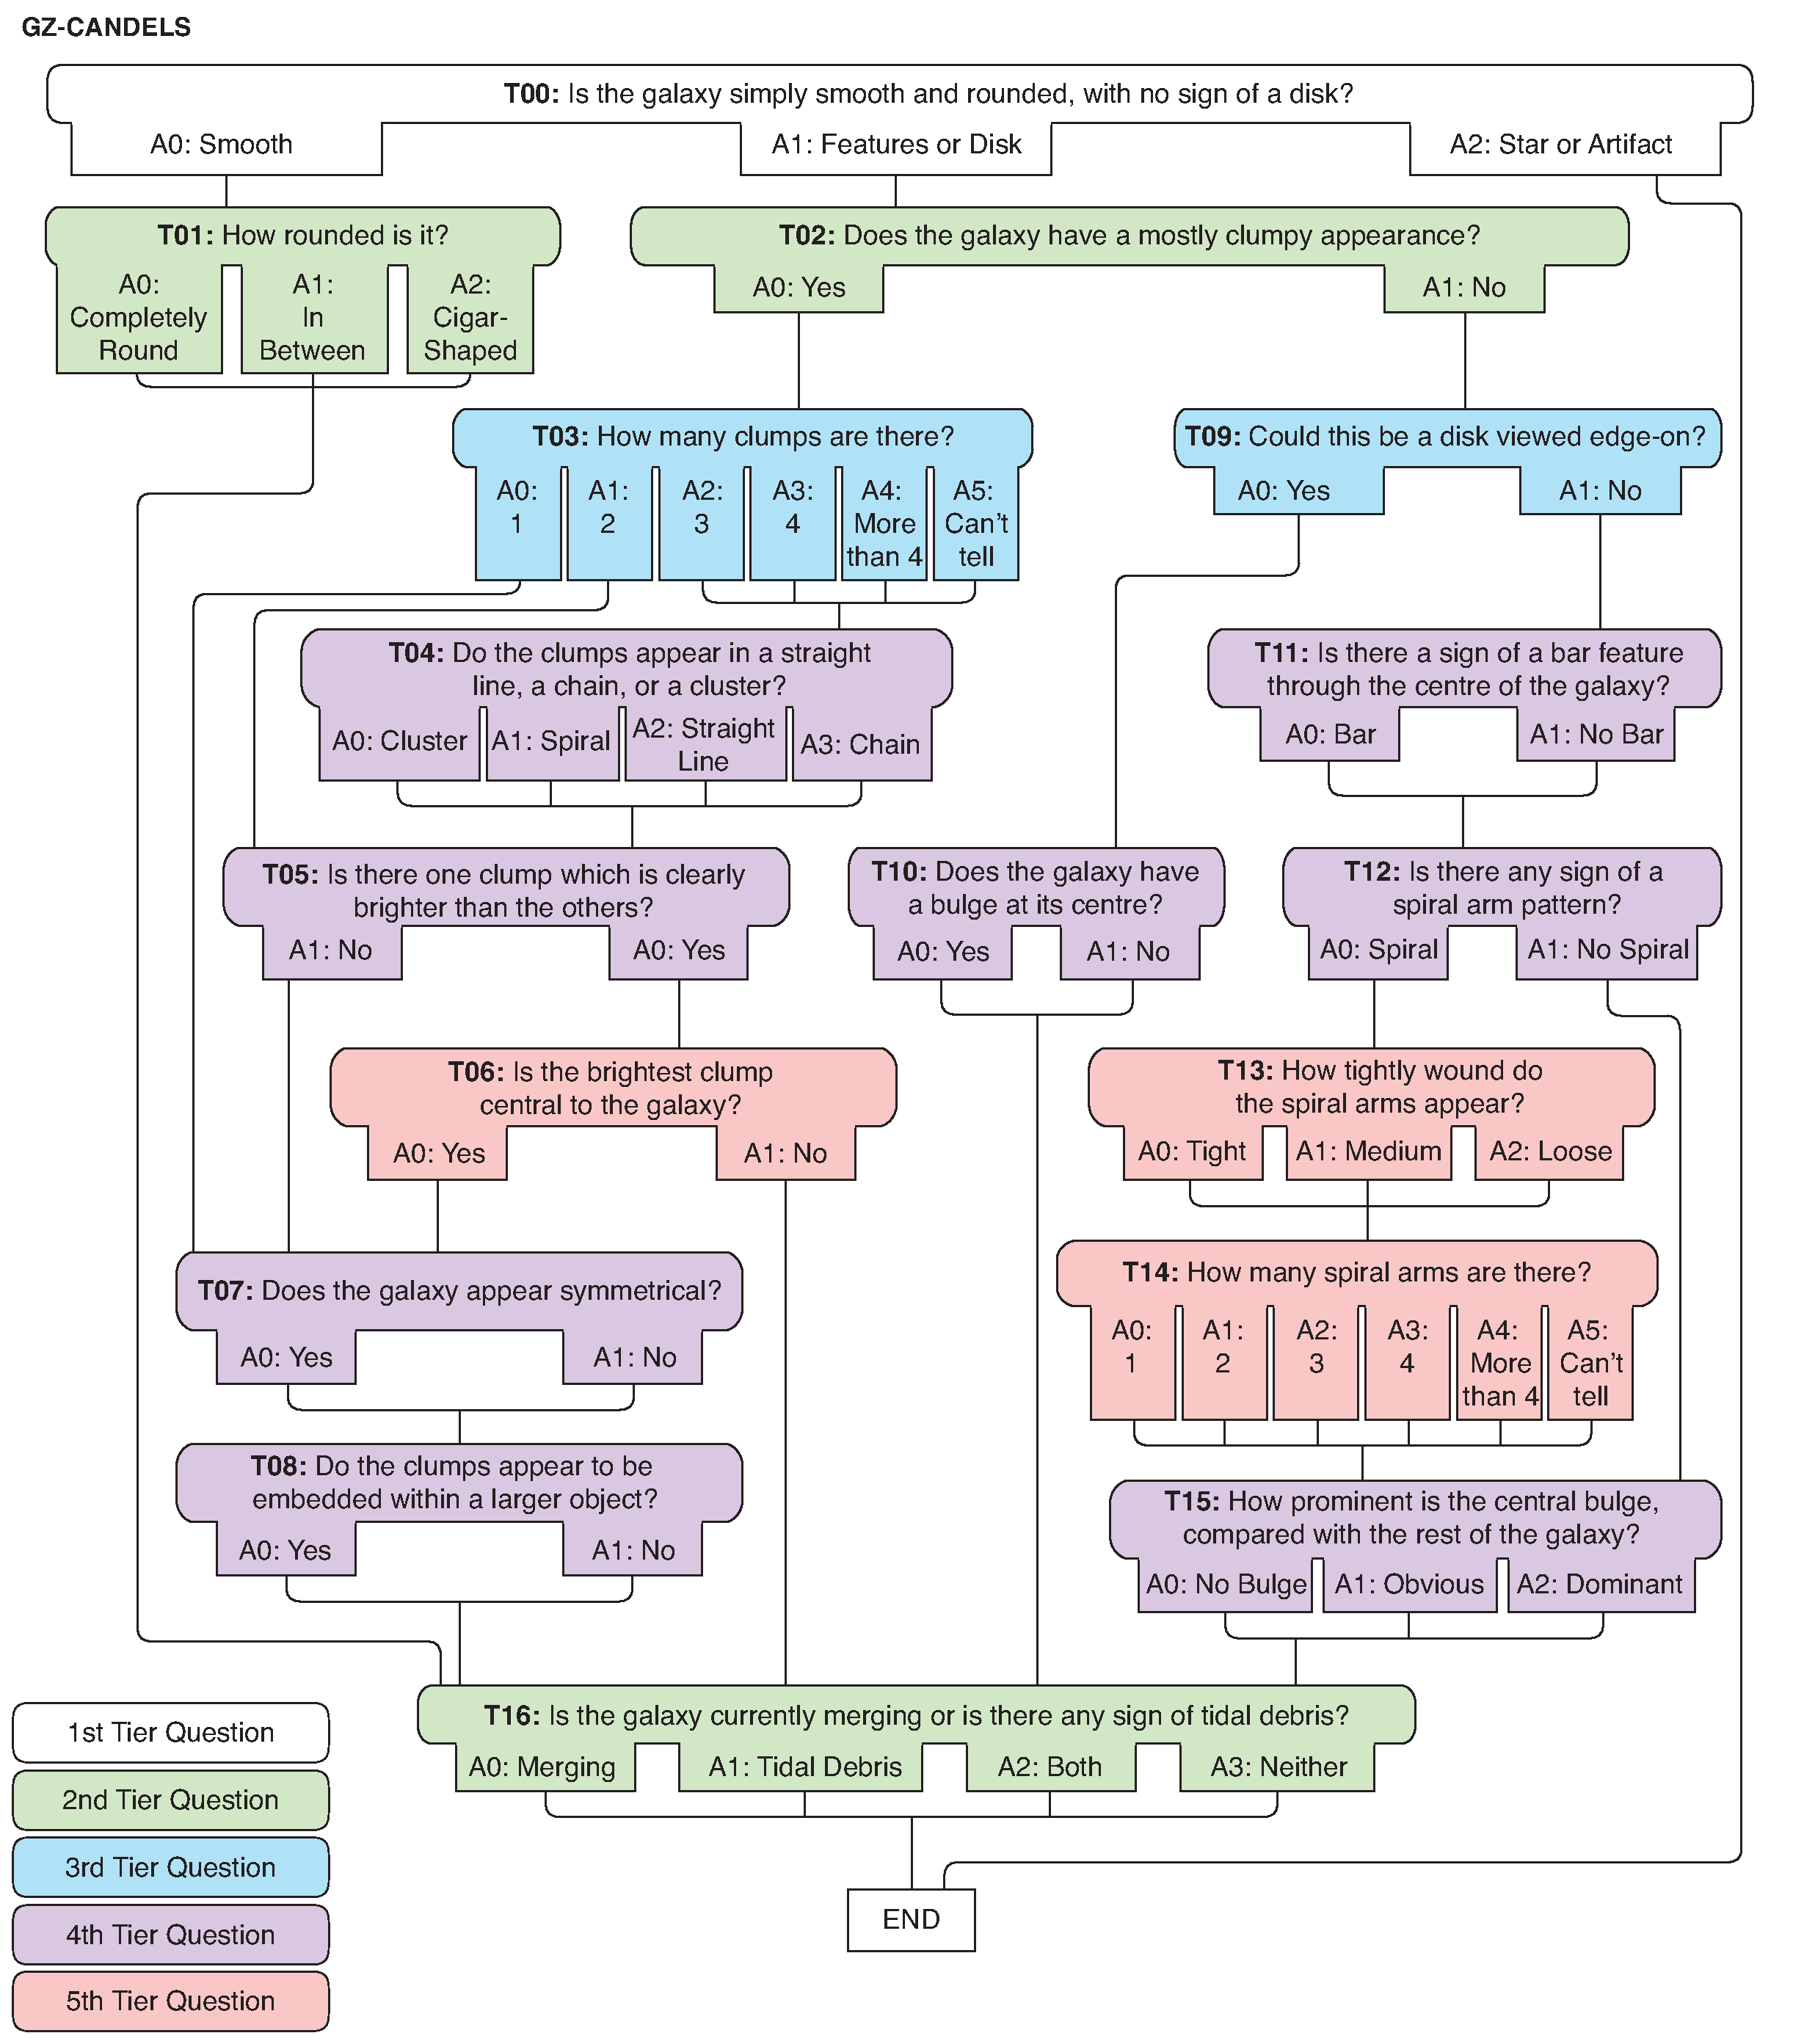
\includegraphics[scale=0.45]{candels_classification_tree_withlabels_new.eps}
\caption{
The Decision Tree for Galaxy Zoo: CANDELS in visual format. There are 16 tasks, with one question per task and up to 6 answers per question. Questions are coloured according to the minimum number of branches prior to that question. All users are asked the first question (task T00), and there are 4 subsequent levels of branching. The tree is also shown in text in Table \ref{table:tree}.
}
\label{fig:tree}
\end{figure*}
%%%%% END FIGURE %%%%%

The goal of Galaxy Zoo CANDELS is to provide detailed quantitative visual morphologies of galaxies observed by the deepest, most complete \emph{HST} multi-wavelength legacy survey to date. 
%The classification interface was designed first and foremost with this goal in mind. 
There are many morphological features of interest, including both broad questions about a galaxy's overall appearance and more detailed questions about specific features. 

We employ a tree-based structure for collecting information on these morphological features, a strategy that has been used successfully in both Galaxy Zoo 2 {\notebsm (refs here)} and Galaxy Zoo: Hubble {\notebsm (and here)}. The decision tree, shown visually in Figure \ref{fig:tree} and in text in Table \ref{table:tree}, first asks the classifier to choose between the broad categories of "smooth and rounded", "features or disk", and "star or artifact". The next question either exits the classification (if the classifier has indicated the image is of a star or artifact) or asks for further details about the galaxy. 

If the classifier has indicated in the first question that the galaxy has features or a disk, a series of follow-up questions are asked about features such as clumps, spiral patterns, bulge strength, and the presence of a bar. If the classifier has instead indicated the galaxy is mostly smooth and rounded, the next question asks them to rate the overall roundedness, a question roughly corresponding to an axis ratio measurement. Finally, when the classifier has finished answering all follow-up questions about either the "smooth" or "featured" galaxy, they are then asked whether the galaxy is undergoing a merger, has tidal tails, or has both, or neither.

The tree-based structure has a number of advantages. First, it collects substantially more information on each galaxy than a single question would, and captures a more detailed classification of higher-order structures while minimising the effort required on the part of the classifier by only asking for relevant inputs based on the answers provided to previous questions. 

Second, it focuses the classifier on a single feature at a time, highlighting each feature. This resets the attention of the classifier with each new question and avoids the problems that may result when a person is presented with a large number of decision tasks at once, including a decrease in optimal decision-making {\notebsm (references for overchoice)} and a reduced ability to recognise the unexpected {\notebsm (references for inattentional blindness)}. 

Third, the tree-based structure is especially optimal for an interface which may collect classifications from users who have never before seen an image of a galaxy and may seek additional training. Within the interface, the classifier may optionally display training images in a ``Help'' section that shows different examples of the feature relevant to the current question. Asking single-topic questions in turn permits a full set of training images to be available throughout the classification without placing an unnecessary cognitive load on the classifier.

%{\notebsm Other advantages we should mention?}

The disadvantage of a tree-based classification structure concerns the dependencies introduced into the vote fractions by such a structure. A classifier cannot, for example, answer that the same galaxy has both a mostly smooth appearance and also has a spiral feature. This is in some ways an advantage, as it prevents contradictory and unphysical classifications, but it also means that an analysis of  morphological vote fractions with the goal of examining spiral galaxies must account for the fact that whether a given classifier reached the spiral branch of the decision tree depends on their answer to the questions preceding it. 

Accounting for dependencies of questions in deeper branches of the decision tree on higher-level questions is, however, a manageable task which has been undertaken successfully in many previous studies of specific galaxy structural features {\notebsm {(for specific examples, see [citation bomb here])}}. 

The Galaxy Zoo CANDELS decision tree is shown in visual form in Figure \ref{fig:tree} and in text form in Table \ref{table:tree}. We note that this tree is most similar to the tree used in the Galaxy Zoo: Hubble project \citep[shown in ][]{melvin14} {\notebsm (note to self to check that the full tree is actually shown there)}, which also has an additional branch identifying clumpy galaxies and focusing on the detailed structure of galaxy clumps. There are small differences, however: for example, Task 10, the question about a bulge in an edge-on disk, is a Yes/No question here, whereas in previous iterations of the decision tree this question also asked whether the bulge shape was rounded or boxy. Additionally, the final question in the tree (Task 16) is substantially different from previous versions and is here only concerned with galaxy mergers and tidal features. 

After the classification of each image is finished, the classifier is asked "Would you like to discuss this object?" If the classifier selects "No", a new image is shown for classification. If the classifier selects yes, a new window opens with a discussion page focused on the image they have just classified. Within this part of the Galaxy Zoo software, called Talk, users may ask questions and make comments on specific images, or engage in more general discussions. Users may also "tag" images and discussions using a format identical to Twitter's hashtag system. Some of these tags were used in the pre-analysis of Galaxy Zoo CANDELS data, on which more details are given in Section \ref{sec:rawclass} below.



\begin{table*}
 \begin{tabular}{@{}cllr}
 \hline
\multicolumn{1}{l}{Task} &
\multicolumn{1}{c}{Question} &
\multicolumn{1}{c}{Responses} &
\multicolumn{1}{c}{Next} 
\\ 
\hline
\hline						
T00    & {\it Is the galaxy simply smooth   }  & smooth           & 01 \\
      & {\it and rounded, with no sign of  }  & features or disk & 02 \\
      & {\it a disk?                       }  & star or artifact & {\bf end} \\
      \hline
T01    & {\it How rounded is it?            }  & completely round & 16 \\
      & {\it                               }  & in between       & 16 \\
      & {\it                               }  & cigar-shaped     & 16 \\
      \hline
T02    & {\it Does the galaxy have a    }  & yes                  & 03 \\
      & {\it mostly clumpy appearance? }  & no                   & 09 \\
      \hline
T03    & {\it How many clumps           }  & 1                    & 07 \\
      & {\it are there?                }  & 2                    & 05 \\
      & {\it                           }  & 3                    & 04 \\
      & {\it                           }  & 4                    & 04 \\
      & {\it                           }  & more than four       & 04 \\
      & {\it                           }  & can't tell           & 04 \\
      \hline
T04    & {\it Do the clumps appear in   }  & cluster              & 05 \\
      & {\it a straight line, a chain  }  & spiral               & 05 \\
      & {\it or a cluster?             }  & straight line        & 05 \\
      & {\it                           }  & chain                & 05 \\
      \hline
T05    & {\it Is there one clump which is       }  & yes          & 06 \\
      & {\it clearly brighter than the others? }  & no           & 07 \\
      \hline
T06    & {\it Is the brightest clump    }  & yes                  & 07 \\
      & {\it central to the galaxy?    }  & no                   & 16 \\
      \hline
T07    & {\it Does the galaxy           }  & yes                  & 08 \\
      & {\it appear symmetrical?       }  & no                   & 08 \\
      \hline
T08    & {\it Do the clumps appear to be       }  & yes           & 16 \\
      & {\it embedded within a larger object? }  & no            & 16 \\
      \hline
T09    & {\it Could this be a disk viewed   }  & yes              & 10 \\
      & {\it edge-on?                      }  & no               & 11 \\
      \hline
T10    & {\it Does the galaxy have a        }  & yes              & 16 \\
      & {\it bulge at its centre?          }  & no               & 16 \\
      \hline
T11    & {\it Is there a sign of a bar      }  & bar              & 12 \\
      & {\it feature through the centre    }  & no bar           & 12 \\
      & {\it of the galaxy?                }                          \\
      \hline
T12    & {\it Is there any sign of a        }  & spiral           & 13 \\
      & {\it spiral arm pattern?           }  & no spiral        & 15 \\
      \hline
T13    & {\it How tightly wound do the      }  & tight            & 14 \\
      & {\it spiral arms appear?           }  & medium           & 14 \\
      & {\it                               }  & loose            & 14 \\
      \hline
T14    & {\it How many spiral arms          }  & 1                & 15 \\
      & {\it are there?                    }  & 2                & 15 \\
      & {\it                               }  & 3                & 15 \\
      & {\it                               }  & 4                & 15 \\
      & {\it                               }  & more than four   & 15 \\
      & {\it                               }  & can't tell       & 15 \\
      \hline
T15    & {\it How prominent is the          }  & no bulge         & 16 \\
      & {\it central bulge, compared       }  & just noticeable  & 16 \\
      & {\it with the rest of the galaxy?  }  & obvious          & 16 \\
      & {\it                               }  & dominant         & 16 \\
      \hline
T16    & {\it Is the galaxy currently       }  & merging          & {\bf end}  \\
      & {\it merging or is there any       }  & tidal debris     & {\bf end}  \\
      & {\it sign of tidal debris?         }  & both             & {\bf end}  \\
      & {\it                               }  & neither          & {\bf end}  \\
      \hline
 \end{tabular}
 \caption{{\notebsm [I'd like to make this a 2-column type table, split after T08, but I don't really have the energy...]} The Galaxy Zoo CANDELS decision tree, comprising 16 tasks and 51 responses. Each task is comprised of a single question and up to 6 possible responses. The first question is Task 00, and a classification is completed by responding to all subsequent questions until the end of the tree is reached. The `Next' column indicates the subsequent task the classifier is directed to upon choosing a specific response. Although a classifier will flow through the tree from top to bottom, there is no path through the tree that includes all tasks. 
%The texts in `Question' and `Responses' are displayed to volunteers during classification, along with the icons in Figure~\ref{fig-flowchart}.
\label{table:tree}}
\end{table*}



\subsection{Raw classifications}\label{sec:rawclass}

% First classification 2012-09-10 18:41:25 UTC, last classification 2013-11-30 12:58:51 UTC
% NOTE I've just discovered that people who put commas in their usernames can mess up my (admittedly simple and awk-based) system of separating classifications. 
% So I am 99% sure the total number of classifications is 2,149,206 but I'm not 100% sure yet.

%%%%% [FIGURE: Example images] %%%%%
\begin{figure*}
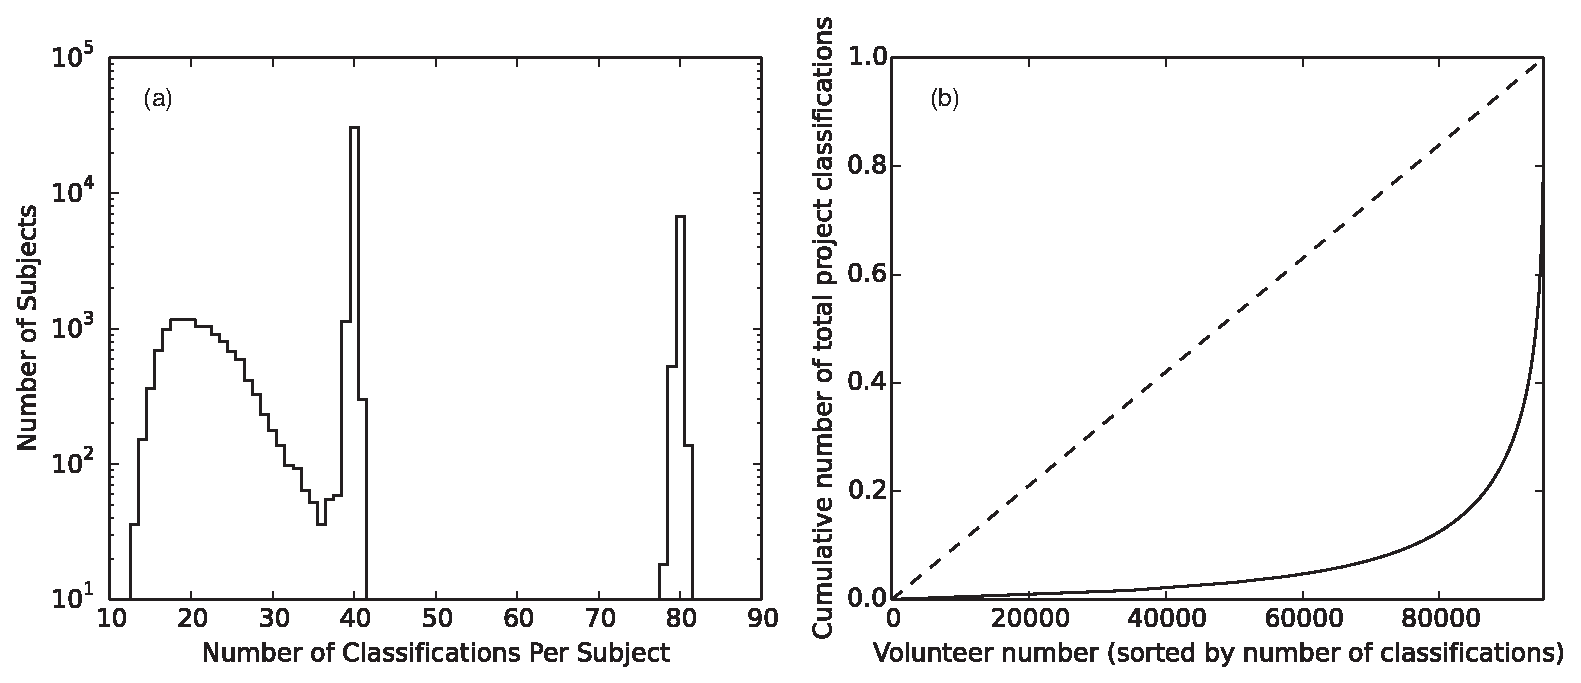
\includegraphics[scale=0.67]{classifications_users_basicinfo.eps}
\caption{
Basic information on classifications. \emph{Left}: Distribution of number of classifications per subject in Galaxy Zoo CANDELS. The majority of images have 40 independent classifications each; a subset of 13,392 were retired early after being identified as too faint and low-surface-brightness for additional classifications to be useful (11,837) or as stars or artifacts (1,555). Subsequently, 7,402 subjects where at least 20\% of classifiers registered a vote for ``Features or Disk'' in the first task were re-activated with a retirement limit of 80 classifications, in order to ensure a complete sampling of the deepest branches of the question tree. \emph{Right}: Cumulative distribution of classifications by volunteers, where the volunteers are sorted in order of least to most classifications contributed (Lorenz curve for classifiers). If every volunteer had contributed the same number of classifications, the Lorenz curve would be equal to the dashed curve. The top 9\% of users contributed 80\% of the classifications (Gini coefficient = 0.86). 
}
\label{fig:classification_basic_info}
\end{figure*}
%%%%% END FIGURE %%%%%


The first classification of an image from CANDELS was registered on the Galaxy Zoo interface\footnote{zoo4.galaxyzoo.org} on the 10th of September 2012. The final classification considered here, in the first phase of Galaxy Zoo CANDELS, was registered on the 30th of November 2013. Between these times, the site collected 2,149,206 classifications of 52,076 CANDELS subjects from 41,552 registered volunteers and 53,714 web browser sessions where the user did not log in. For all analysis presented here we have assumed that each unregistered browser session contains classifications from a single, unique volunteer. 

Subjects within a given Galaxy Zoo sample are chosen randomly for classification, so that the number of independent classifications per galaxy builds up uniformly through the full sample. Once a pre-set classification limit has been reached, the subject is retired from the active classification pool. The initial goal for Galaxy Zoo CANDELS was to obtain at least 40 independent classifications for each galaxy. 

This uniform retirement limit was modified twice during the project. In the first instance, a pre-analysis of the dataset performed when the average number of classifications per galaxy had reached approximately 20 revealed 11,837 subjects where further classification was unlikely to provide any additional information. These subjects were identified with the help of a set of subjects tagged in the Galaxy Zoo Talk software as ``\#toofainttoclassify'' and ``\#FHB'' (which stands for ``Faint Hubble Blob''). Tags in Galaxy Zoo Talk are generally highly incomplete; thus the 204 tagged subjects were used as tracers during a further examination of all subjects in magnitude-surface brightness parameter space. The selection, made from initial photometry, was deliberately conservative, retiring only those subjects where it was clear that the classification vote fractions had converged at all tiers of the classification tree. During this analysis, an additional 1,555 subjects were identified as highly likely to be stars or artifacts and were also retired.

The second modification of the retirement limit was implemented 1 year after the project start. At this time, the retirement limit was raised to 80 classifications for all galaxies where at least 20\% of volunteers had answered ``Features or Disk'' to the first question (task T00 in Figure \ref{fig:tree} and Table \ref{table:tree}). This is a higher retirement limit than in previous Galaxy Zoo projects, and it is justified by the increased complexity of the question tree compared to, e.g., Galaxy Zoo 2 \citep{willett13}. The Galaxy Zoo CANDELS question tree has an additional branch level, and the number of volunteers answering a question is typically reduced at each branch point. Thus, 40 classifications at the first question may not be enough to ensure convergence in, for example, task 14, ``How many spiral arms are there?'', a 5th-tier question with 6 possible answers. The increased retirement limit affected 7,402 subjects.

Figure \ref{fig:classification_basic_info}a shows the distribution of total classification counts within the sample. The majority of subjects received 40 classifications, but the distribution is asymmetric: there are peaks at $\sim 20$, $40$, and $80$ classifications, consistent with the description above. The Lorenz curve of classifications by volunteers is shown in Figure \ref{fig:classification_basic_info}b. The curve is highly skewed from the $1:1$ line that would be seen if all volunteers contributed the same number of classifications; the top 9\% volunteers contributed 80\% of total classifications. The Gini coefficient for classfications, i.e., the fractional difference in area under the Lorenz curve versus the dashed line, is 0.86. This is typical of past Galaxy Zoo projects and Zooniverse\footnote{zooniverse.org} citizen research projects in general {\notebsm (could cite VOLCROWE CiSE paper here)}. 

The values in Figure \ref{fig:classification_basic_info} are raw classification counts; while raw classification counts and vote fractions are certainly useful, we additionally apply a user weighting scheme to classifications to produce a cleaner set of vote fractions for each subject. The user weighting is described in further detail below.



\subsection{User Weighting} \label{sec:weighting}

% If we're not talking about IBCC then we don't need to distinguish this.
%\subsubsection{Consensus Weighting}

Multiple methods of user weighting have been successfully employed by many different Zooniverse projects {\notebsm \citep{lintott08, bamford09, lintott11, esimpson12, rsimpson12, johnson15, marshall15}}. In general, the optimal choice of user weighting depends on the amount of information available per subject and the goal of the project. In Galaxy Zoo CANDELS the goal is to converge to a classification for each galaxy whilst still allowing for unexpected discoveries, and there is ample information from classifiers but little information on the ``ground truth'', i.e., we do not know what the true intrinsic classification is for even a modest fraction of the sample.

For these reasons, we adopt an iterative consensus-based weighting method, following previous Galaxy Zoo projects. This weighting scheme effectively identifies the small proportion of classifiers whose contributions are routinely errant compared to other classfiiers (or consistent with random inputs) and downweights their contributions, while preserving the inputs from the vast majority of users.

Weights for each user are computed based on a mean consistency factor, \kappamean , which is the average of consistencies for each of that user's classifications. For a given classification $i$ composed of a series of completed tasks $t$ answered about a specific subject, we compare the user's answer to each task with the aggregated classifications of other users of the same subject. Each task has $a_t$ answers from all users, each of which is assigned to one of $N_{r,t}$ possible responses to the task. We define the vote fraction for a particular response $r$ as $f_r \equiv a_r/a_t$, where $a_r$ is the number of positive answers for that response (i.e., the number of classifiers who selected that response out of all possible responses to the task).

For each task that was completed by the classifier in classification $i$, the consistency index $\kappa_r$ for each response $r$ to that task $t$ is 
\begin{equation}
    \kappa_r = \left\{
    \begin{array}{l l}
      f_r       & \text{ if the classifier's answer corresponds} \\
                  & \text{ to this response,}\\
      (1 - f_r) & \text{ if the answer does not correspond.}\\
    \end{array} \right.
    \label{eqn-consistency-r}
 \end{equation}
The consistency for that task, $\kappa_t$, is the average of these indices over all possible responses. For example, if a classifier responded ``Star or Artifact'' to Task T00 for a particular subject, and the overall vote fractions on that task for that subject are $($``Smooth'', ``Features or Disk'', ``Star or Artifact''$) = (0.1, 0.6, 0.3)$, then the user's consistency for Task T00 for this classification is
$$
\kappa_t = \left[\left(1 - 0.1\right) + \left(1 - 0.6\right) + 0.3\right]/3 = 0.5\overline{3}.
$$
In the above example, the user's answer to Task T00 leads to the end of the workflow (Table \ref{table:tree}), so this $\kappa_t$ is also equal to the user's consistency for the overall classification, $\kappa_i$. More generally, the classification consistency is the answer-weighted average of the task consistencies:
\begin{equation}
\kappa_i = \frac{\sum_t \kappa_t a_t}{\sum_t a_t} ,
\label{eqn-consistency-i}
\end{equation}
where each sum is over the number of tasks the user completed during the classification.

Following this calculation for the entire classification database, each user's average consistency is calculated as
\begin{equation}
\mkappamean = \frac{1}{N_i} \sum_i \kappa_i .
\label{eqn-consistency-avg}
\end{equation}

Averaging over a user's individual consistency values for all classifications effectively downweights those contributions from users whose classifications regularly diverge from the consensus whilst preserving the diversity of classifications from volunteers who are \emph{on average} consistent with each other. It also allows for the classifications of skilled volunteers to remain highly weighted even on difficult subjects where the individual consensus is skewed (e.g., if an image is very noisy or if a nearby artifact is distracting to less experienced volunteers). 

The user weight is then calculated as 
\begin{equation}
w = \min \left(1.0,(\mkappamean / 0.6)^{8.5} \right) ,
\label{eqn-weight}
\end{equation}
a formulation that preserves a uniform weighting for any classifier with $\mkappamean \geq 0.6$ and downweights those with a lower consistency rating.

The weighted consensus classifications are then calculated for each subject by summing the weighted votes for each task and response, and reporting the vote fractions $f$ for each. As the user weights are calculated via comparison with the consensus, which leads to a new consensus, this method can be iterated until the user weights converge to a stable value. 

In practice, the number of iterations required to reach this goal is low \citep[e.g., 3 or less in previous projects;][]{bamford09,willett13}. In Figure \ref{fig:consistencies} we show the distribution of user consistencies after 1, 2 and 3 iterations of the above method. Approximately 3 per cent of users have consistency $\mkappamean < 0.5$ (corresponding to a weight $w \lesssim 0.2$), whereas 85 percent of users have an end weight of $w = 1$. The vast majority of Galaxy Zoo volunteers contribute highly valuable information to the project.

%%%%% [FIGURE: Example images] %%%%%
\begin{figure}
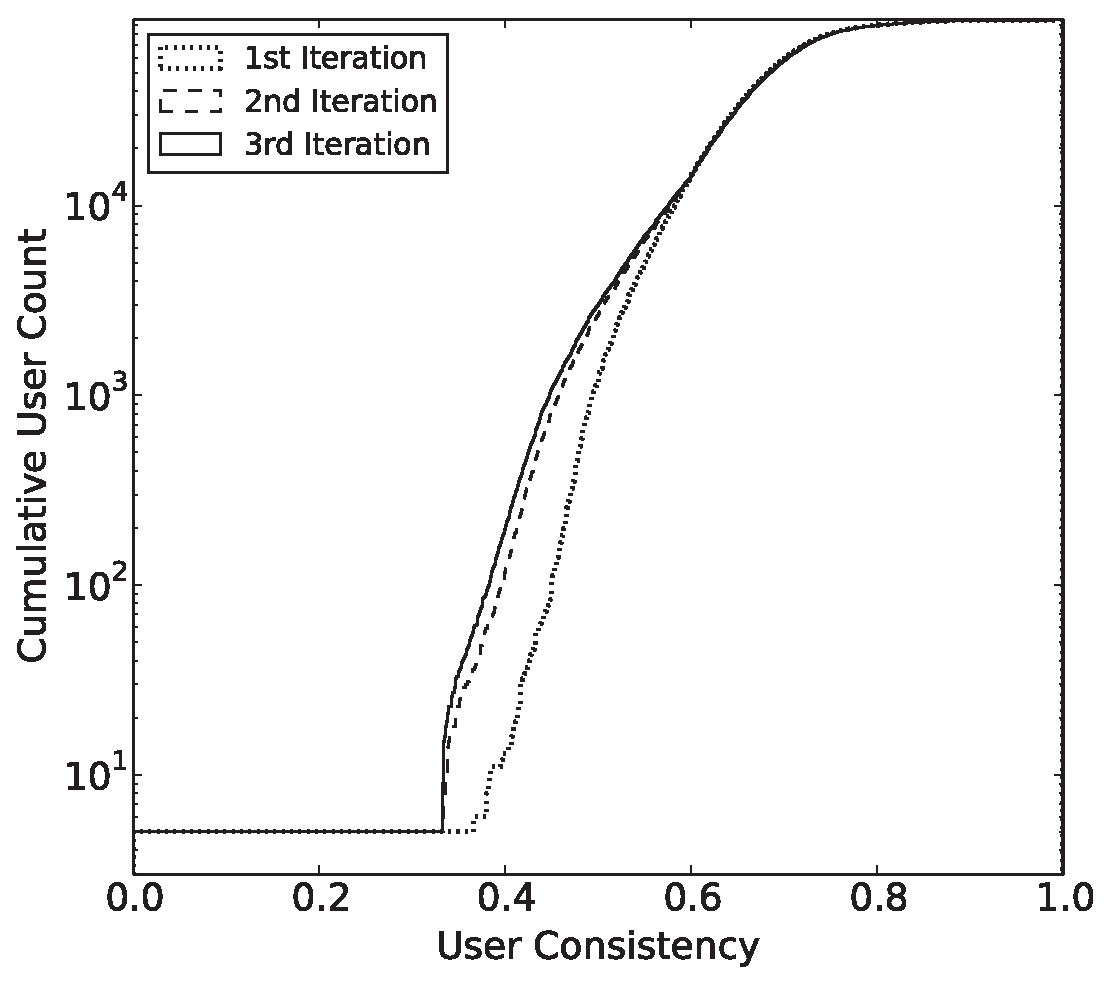
\includegraphics[scale=0.465]{consistencies_iterations.eps}
\caption{
Distribution of user consistencies \kappamean\ after 1 (dashed), 2 (dotted), and 3 (solid) iterations of the consistency-based weighting method  (described in Section \ref{sec:weighting}). Convergence of this method requires relatively few iterations: further iterations do not change significantly from the solid curve. Approximately 85 per cent of users have $\mkappamean \geq 0.6$ and weights $w = 1$. 
}
\label{fig:consistencies}
\end{figure}
%%%%% END FIGURE %%%%%


% Postponing this as the IBCC classifications are a little weird - we need a bigger training set.
%\subsubsection{IBCC}


\subsection{Depth, Surface Brightness, and Classification Bias}\label{sec:biases}

The consistency-based weighting described above ensures the preservation of the way in which the variety of volunteer classifications echoes the confidence level in any individual response, while ensuring expert classifiers remain highly weighted and the very small fraction of errant classifiers are down-weighted.

However, the amount of information available per subject varies: the CANDELS survey takes images at multiple depths, and the galaxies themselves have a wide range of intrinsic brightnesses and distances. Even at a given redshift, the classification of a galaxy depends on both its luminosity and size (i.e., its surface brightness). In particular, as the observed surface brightness of a galaxy decreases it tends to appear more smooth compared to the image noise, decreasing the detection of features \citep{bamford09,willett13}.

Previous Galaxy Zoo projects examining galaxies in the more local Universe have accounted for this bias by using less distant galaxies to determine how to debias the classifications of more distant galaxies as a function of redshift. This is effective under the assumption that the underlying distribution of classifications is invariant with redshift. Clearly this is an inappropriate assumption in the case of a deep \emph{HST} survey such as CANDELS, where 80 per cent of subjects fall within the redshift range $0.25 < z < 3.5$, over which galaxy shapes most certainly evolve.

Despite these challenges, Galaxy Zoo volunteers have proven extremely reliable at classifying features which are visible above some surface brightness detection limit. When the overall surface brightness of a galaxy falls below that limit, the detection of locally more bright features may still be achieved, but in general the classification vote fraction of a galaxy as ``featured'' may be considered a lower limit. We describe below the determination of a surface brightness limit for Galaxy Zoo CANDELS and discuss its implications for usage of the vote fractions.


\subsubsection{Surface brightness limits in Galaxy Zoo CANDELS}

We aim to determine empirically the surface brightness threshold above which Galaxy Zoo CANDELS classifications reliably characterise the level of ``features'' present in a galaxy. It is therefore important to choose a subset of galaxies so as to minimise the dependence of a galaxy's ``true'' classification on factors such as distance and luminosity.

We define the observed surface brightness of a galaxy using the magnitude and size reported in the CANDELS photometric catalogs for each field \citep[][Peth et al., in preparation]{guo11,fill_in,later}. Specifically, we use the $F160W$ \textsc{auto} fluxes and the radius containing 80\% of the galaxy light, $r_{80}$, to determine a representative surface brightness for each galaxy. We also use the measured axis ratios $b/a$, dividing the flux by the area contained within an ellipse of area $\pi a_{80} b_{80}$, in square arcseconds. We then convert to magnitudes, resulting in a single surface brightness $\mu_{\textsc{auto}}$ in mag/arcsec$^2$ for each subject. 

We then choose a subset of subjects from the full sample described above within a narrow range of redshifts to minimise evolutionary effects. We use galaxies with $1.1 < z < 1.4$, spanning an evolutionary period of $\sim 1$~Gyr, but note the analysis is insensitive to the specific choice of redshifts so long as the bin spans a similar time period.

Figure \ref{fig:sb_z1} shows the vote fractions for the response ``Features or Disk'' in the first question (task T00) in the decision tree, versus surface brightness. The variation in the distribution of featured classifications with surface brightness is apparent even after disregarding subjects with $\mu_{\textsc{auto}} < 20$~mag/arcsec$^2$, which are typically stars. The right panel of Figure \ref{fig:sb_z1} shows these distributions as cumulative histograms binned by $\Delta \mu_{\textsc{auto}}$. As expected, the distribution of featured vote fractions changes with surface brightness, with all vote fraction distributions being similarly lacking in detected features for observed $\mu_{\textsc{auto}} > 23.0$~mag/arcsec$^2$.  

Therefore, although we report vote fractions for all subjects in the Galaxy Zoo CANDELS catalog, including those with $\mu_{\textsc{auto}} > 23$, we strongly urge caution when using classifications of galaxies fainter than this surface brightness level. Featured vote fractions at surface brightnesses fainter than this may be reasonably considered lower limits, as many features may not be visually apparent. In all subsequent analysis in this paper, we consider only galaxies with $\mu_{\textsc{auto}} < 23.0$ unless otherwise specified. 


%%%%% [FIGURE: Example images] %%%%%
\begin{figure*}
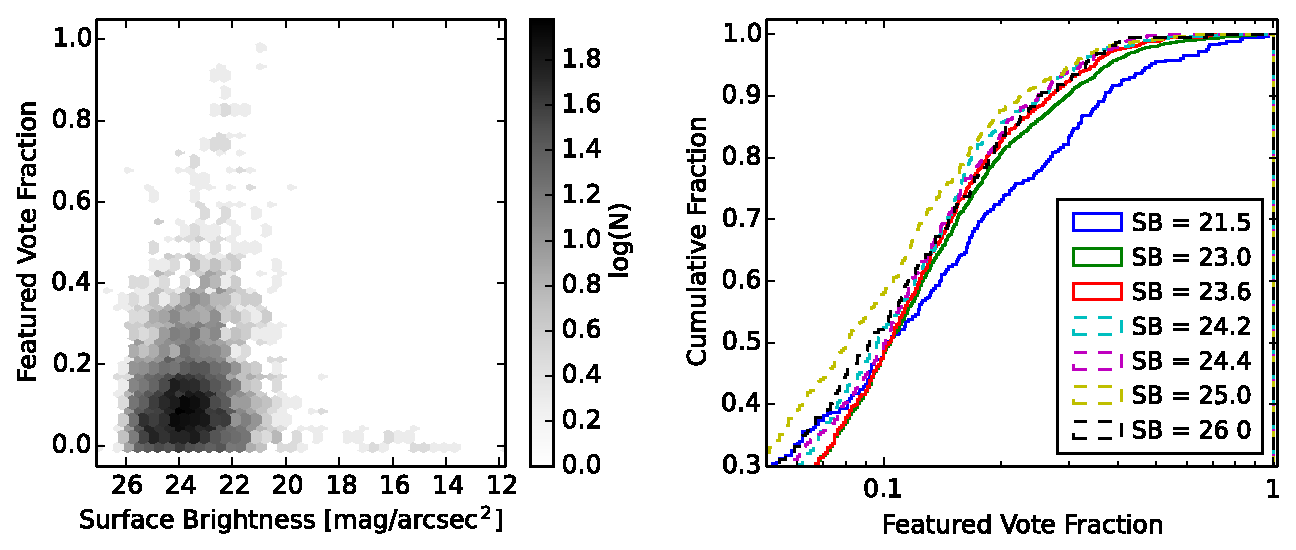
\includegraphics[scale=0.8]{sb_z1.eps}
\caption{
Comparison of subject surface brightnesses and vote fractions for the response ``Features or Disk'' in the first task (T00) of Galaxy Zoo CANDELS for subjects with $1.1 < z < 1.4$. \emph{Left:} 2-D histogram of $f_{\rm features}$ versus $\mu_{\textsc{auto}}$, with shading of each hexagonal bin indicating the number of subjects in that bin. Subjects with  $\mu_{\textsc{auto}} < 20$~mag/arcsec$^2$ are generally point-like sources. The distribution of featured vote fraction is a function of surface brightness. \emph{Right:} Cumulative distributions of $f_{\rm features}$ in bins of surface brightness. Although we note that some of the variations seen are likely due to intrinsic differences in populations at different luminosities, there is a clear and strong change in the distribution at $\mu_{\textsc{auto}} \approx 23.0$. 
}
\label{fig:sb_z1}
\end{figure*}
%%%%% END FIGURE %%%%%



%\subsubsection{The effect of image depth on classifications}

%Old words
%80 per cent of all subjects in Galaxy Zoo CANDELS have redshifts $0.25 < z < 3.5$, over which cosmological distances galaxies of identical luminosities will have observed fluxes that differ by orders of magnitude. The angular diameter distance, meanwhile, varies in a very different way (and indeed does not evolve much beyond $z \sim 1$ compared to the luminosity distance). 


\subsection{Use of Classifications in Practice}\label{sec:usage}

The branched nature of the decision tree (Figure \ref{fig:tree}) means that selection of a sample of galaxies for a given morphological investigation may depend on a number of factors. For example, it is possible to choose a quantitative threshold for selection of a sample of galaxies with a given feature or combination of features corresponding to one's optimal trade-off between sample completeness and purity. One may also weight a population analysis by the vote fraction for a particular morphological feature (making the assumption that the probability of a galaxy having that feature, or the strength of the feature, is a function of the vote fraction). However, for all tasks below T00 in the tree, it is important to consider the responses to the tasks above that question in this analysis.

For example, a study with the goal of examining spiral galaxies would ideally use a sample selected by considering the responses to task T12, ``Is there any sign of a spiral arm pattern?'' If a pure sample of galaxies with clear spiral arms is desired, a threshold may be selected at a high vote fraction for $f_{\rm spiral}$. If the threshold considers only this vote fraction, however, the final sample will likely be contaminated by galaxies where the spiral vote fraction is dominated by noise because only a small number of people reached that task (e.g., a warped edge-on disk). 

In order to reach task T12, a user must give specific answers to the questions ``Is the galaxy simply smooth and rounded, with no sign of a disk?'' (T00), ``Does the galaxy have a mostly clumpy appearance?'' (T02), and ``Could this be a disk viewed edge-on?'' Each of these classifications should be considered in the context of the study's goals in order to select as pure a sample as possible whilst minimising contamination and bias.

If a moderately complete sample is desired, for example, the user could select thresholds for the selection such as $f_{\rm features} > 0.5$, $f_{\rm not\ clumpy} > 0.5$, $f_{\rm not\ edge-on} > 0.5$. Because most galaxies with these classifications will have received 80 classifications apiece (Section \ref{sec:rawclass}), these chained thresholds mean the minimum number of volunteers who will have answered the spiral question is $80 \times 0.5^3 = 10$. Higher thresholds will further restrict the minimum number of respondents to the deeper-branched question. If lower thresholds are desired, we recommend that the selection explicitly require a minimum number of respondents to each task. 

There is no single set of thresholds that is ideal for all situations. However, in the data release accompanying this paper, we include ``clean'' selections of galaxies with different morphological features. These are detailed further below, but we additionally encourage users of this rich data set to experiment with different threshold/weight combinations in order to achieve their scientific goals.

\subsection{Data release and ``clean'' samples}

This paper includes the release of the raw and weighted classifications for each of the $49,555$ subjects in the Galaxy Zoo CANDELS sample. In addition to each raw and weighted vote fraction for each task, we include the raw and weighted number of answers to each task, as well as for the whole galaxy overall. This combines for a total of 136 quantities for each subject, not including the subject ID or any other metadata. Clearly this is too much information to present a sample table in print here. However, the data is structured thusly for each task number $NN$ with $i = {0 {\rm\ to\ } n-1}$ responses:
%oh god it's really late and I just said "thusly"

\begin{itemize}
\item[] \small{\tt t[$NN$]\_[quest\_abbrev]\_a[$i$]\_[resp\_abbrev]\_frac} : the raw fraction of users who gave this response. {\tt quest\_abbrev} and {\tt resp\_abbrev} are abbreviated versions of the specific question and response, respectively.

\item[] \small{\tt t[$NN$]\_[quest\_abbrev]\_a[$i$]\_[resp\_abbrev]\_weighted\_frac} : the weighted fraction of users who gave this response. 

\item[] \small{\tt t[$NN$]\_[quest\_abbrev]\_count} : the raw count of users who responded to this task. 

\item[] \small{\tt t[$NN$]\_[quest\_abbrev]\_weight} : the weighted count of users who responded to this task. 

\end{itemize}

For example, the information available for task T00, which has 3 responses, is structured as:

\begin{itemize}
\item[] \small{\tt t00\_smooth\_or\_featured\_a0\_smooth\_frac}

\item[] \small{\tt t00\_smooth\_or\_featured\_a1\_features\_frac}

\item[] \small{\tt t00\_smooth\_or\_featured\_a2\_star\_or\_artifact\_frac}

\item[] \small{\tt t00\_smooth\_or\_featured\_a0\_smooth\_weighted\_frac}

\item[] \small{\tt t00\_smooth\_or\_featured\_a1\_features\_weighted\_frac}

\item[] \small{\tt t00\_smooth\_or\_featured\_a2\_star\_or\_artifact\_weighted\_frac} 

\item[] \small{\tt t00\_smooth\_or\_featured\_count} 

\item[] \small{\tt t00\_smooth\_or\_featured\_weight}

\end{itemize}

The sum of raw  {\tt \_frac} fractions adds to 1.0, as does the sum of {\tt \_weighted\_frac} fractions. Multiplying the {\tt \_frac} values (raw fractions) by the {\tt \_count} (raw user counts) will retrieve the number of people who gave a specific response; likewise with weighted answer counts from {\tt \_weighted\_frac} and {\tt \_weight}. As the user weighting described in Section \ref{sec:weighting} assigns a weight of $w \leq 1$ to each classifier, the weighted vote count must be less than or equal to the raw vote count. While the raw vote counts and fractions are provided for completeness, we recommend that users of this data set use the weighted fractions and counts.

In addition to the vote fractions for each subject, we provide a set of flags for each subject that indicates its member or non-member status in a ``clean'' sample of galaxies of a specific type. We select separate clean samples of smooth, featured, clumpy, edge-on, and spiral galaxies. These samples contain exemplars of each galaxy type with minimal contamination of the sample, and are correspondingly highly incomplete. They are selected according to the following thresholds using weighted vote fractions:

\begin{itemize}

\item[] \textbf{Smooth} - Task T00: $f_{\rm smooth} > 0.9$, $f_{\rm star\ or\ artifact} < 0.2$

\item[] \textbf{Featured} - Task T00: $f_{\rm features} > 0.9$, $f_{\rm star\ or\ artifact} < 0.2$

\item[] \textbf{Clumpy} - Task T00: $f_{\rm smooth} > 0.9$, $f_{\rm star\ or\ artifact} < 0.2$; Task T02: $f_{\rm clumpy} > 0.8$

\item[] \textbf{Edge-on} - Task T00: $f_{\rm smooth} > 0.9$, $f_{\rm star\ or\ artifact} < 0.2$; Task T02: $f_{\rm not\ clumpy} > 0.5$; Task T09: $f_{\rm edge-on} > 0.7$

\item[] \textbf{Spiral} - Task T00: $f_{\rm smooth} > 0.9$, $f_{\rm star\ or\ artifact} < 0.2$,; Task T02: $f_{\rm not\ clumpy} > 0.5$; Task T09: $f_{\rm not\ edge-on} > 0.7$; Task T12: $f_{\rm spiral} > 0.8$

\end{itemize}


We provide these flags for the convenience of the end user, but we additionally encourage those wishing to use Galaxy Zoo classifications to investigate whether a different set of thresholds would be optimal for their own science case.

%%%%%%%%%%%%%%%%%%%%%%%%%%%%%%%%%%%%%%%%%%%%%%
%
%  
\section{Comparison to other visual classifications}\label{sec:comparison}
%
%
%%%%%%%%%%%%%%%%%%%%%%%%%%%%%%%%%%%%%%%%%%%%%%

Most of the galaxies in the CANDELS data set have additional visual classifications available in the form of expert classifications from astronomers and students who are members of the CANDELS team. Analysis of the full set of classifications in that separate project is still underway; the first release of classifications from the GOODS-South field is presented by \citet{kartaltepe14}, hereafter K14, who also detail the project design and objectives, including the classification interface. Consensus classifications from the UDS field are also available {\notebsm (Kartaltepe et al., in preparation)}. For each galaxy in all fields, between 3 and 7 (typically 3) members of the CANDELS team provided classifications.

The classification scheme described in K14 is substantially different to that presented here. Firstly, while that project collects detailed classifications about a number of possible structural features (with 37 different responses possible), they do not always align precisely with the questions asked in Galaxy Zoo CANDELS. For example, the Main Morphology Class of K14 requires the user to select at least one option from among ``Disk'', ``Spheroid'', and ``Peculiar/Irregular'' galaxy types, along with options for ``Point Source/Compact'' and ``Unclassifiable''. The last of these is not an option Galaxy Zoo provides, and the first two are not necessarily the same as task T00's responses of ``Features or Disk''. While Galaxy Zoo does ask about bulges, it does so after multiple branches of the decision tree, and therefore this is not easily comparable to a 1st-tier question.

In fact, \emph{all} responses collected by the CANDELS team interface are 1st-tier questions: the user is presented with all 37 options at once. Additionally, colour composites are not used in that project. Images from each ACS and WFC3 filter are presented separately within the interface, with an option for the user to specify when classifications differ significantly between filters. Users may also view the segmentation map in the $F160W$ band, and in the Perl/DS9 version of the CANDELS team interface the user may adjust the stretch of the image as well. These options are not available to Galaxy Zoo volunteers. On the other hand, the Galaxy Zoo decision tree asks multiple questions designed to elucidate the configuration of clumps in a galaxy, whereas the CANDELS team interface does not. 

Despite these significant differences, it is nevertheless helpful to compare the CANDELS team classifications to the Galaxy Zoo CANDELS classifications. Figure \ref{fig:candels_compare} shows the comparison of vote fractions in four categories: Featured, Merger or Interaction, Edge-On, and Barred. For all comparisons below we have compared the subset of sources in CANDELS above the surface brightness limit described in Section \ref{sec:sblimits} which have visual classifications from both teams, which have \emph{not} been deemed ``unclassifiable'' by the CANDELS team, and which have \emph{not} been rejected as stars or artifacts by more than 50\% of classifiers for either project.
  
%%%%% [FIGURE: Example images] %%%%%
\begin{figure*}
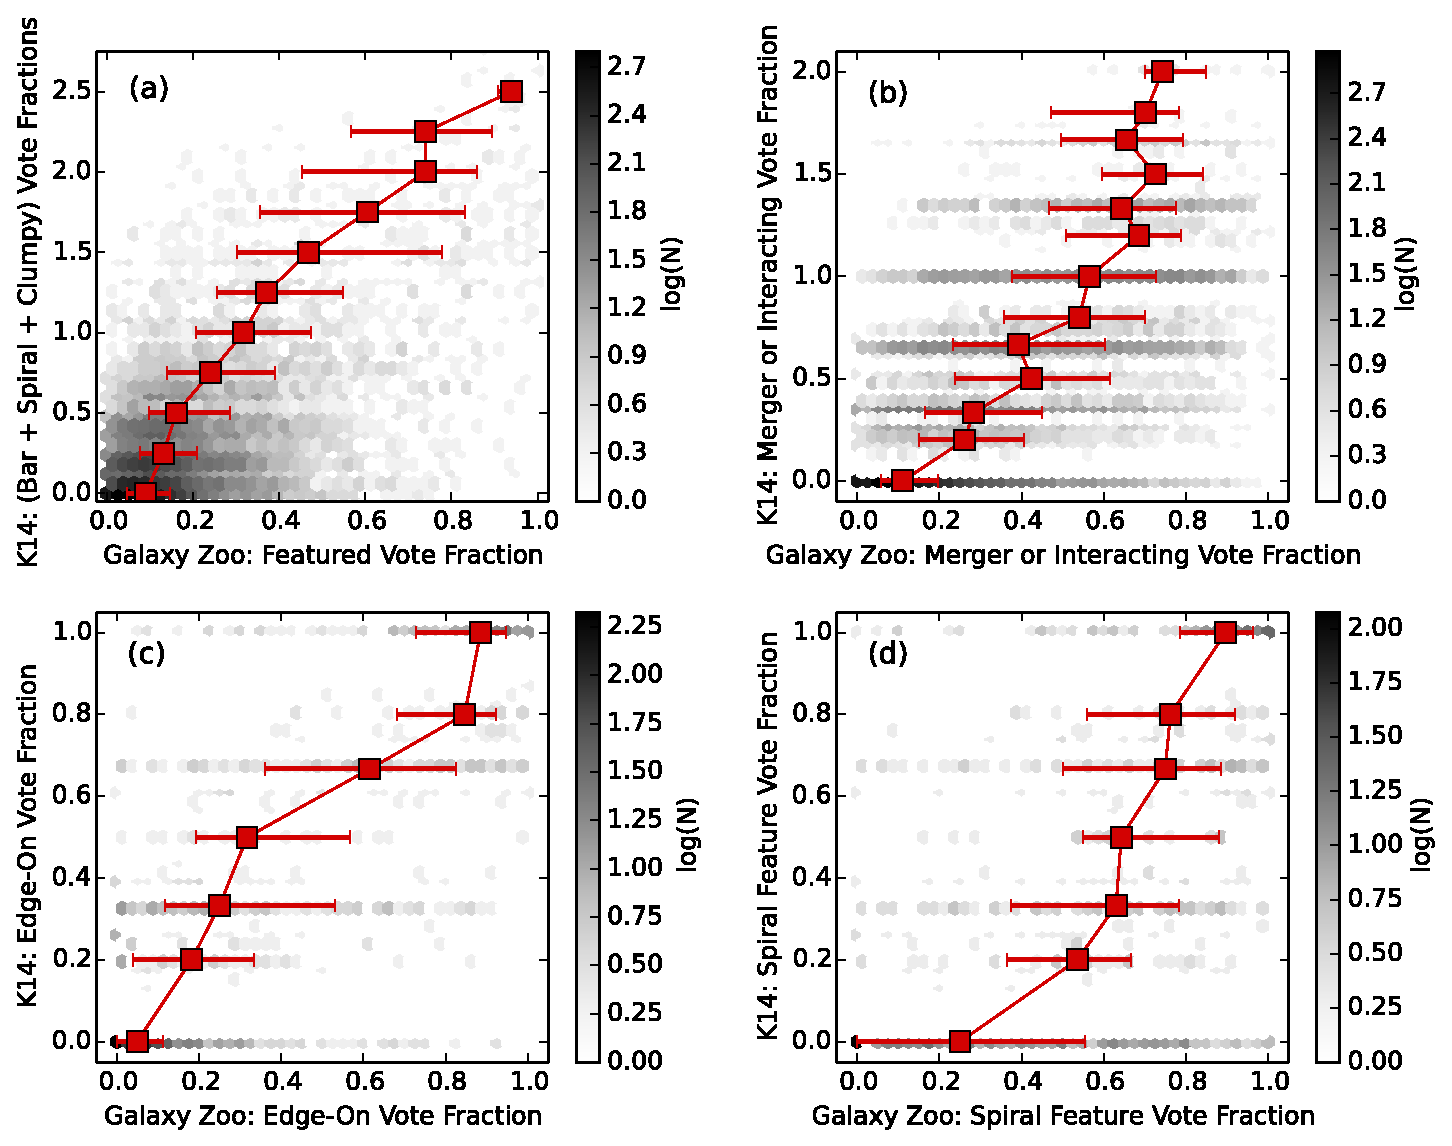
\includegraphics[scale=0.65]{gzteam_candelsteam_multiplot_compare2.eps}
\caption{
Comparison of Galaxy Zoo classifications with visual classifications from the CANDELS team \citep[][K14]{kartaltepe14}. The classification questions differ between the two projects, but we have selected 4 different classifications which are the most similar: (a) the sum of vote fractions in K14 for spiral, bar, and clumpy features, versus the Galaxy Zoo vote fraction for ``Features or Disk'' in task T00. Note that the sum of these vote fractions from K14 can add to $> 1$; (b) vote fractions for merger or interactions (task T16 in the Galaxy Zoo decision tree) for those subjects not identified as ``Star or Artifact'' in task T00; (c) vote fractions for the presence of an edge-on disk (task T09) for subjects that are neither artifacts nor predominantly smooth, nor dominated by clumps; and (d) vote fractions for the presence of spiral arms (task T12) for those subjects in panel (c) that are not edge-on. In all panels, the number of individual galaxies in a given hexagon in parameter space is shown by its shaded value. Red squares show the median Galaxy Zoo vote fraction and within a given K14 vote fraction bin; error bars show the interquartile region (from the 25th to 75th percentile). The different visual classification methods track each other well across many different kinds of structural classification.
}
\label{fig:candels_compare}
\end{figure*}
%%%%% END FIGURE %%%%%

\subsection{Featured Galaxies}

We seek to compare the overall classification of CANDELS galaxies as ``smooth'' or ``featured'' between Galaxy Zoo and the CANDELS team. However, the team interface described in K14 does not specifically ask about this distinction. It does ask about disks and spheroids; however, equating ``smooth'' to ``spheroid'' and ``featured'' to ``disk'' requires assumptions about galaxies at $z > 1$ that we would prefer to avoid.

We therefore compare the ``Features or Disk'' vote fraction for T00 in Galaxy Zoo CANDELS to a combination of vote fractions from the CANDELS team classifications. We choose a set of structures that are unambigously inconsistent with a smooth light distribution in a galaxy, namely spiral arms, clumps, and bar features. 

Within the CANDELS team classification interface, a user may indicate the presence of a bar or spiral arms by selecting one response for each, $f_{\rm bar, \textsc{ct}}$ or $f_{\rm spiral, \textsc{ct}}$. The clumpy classification, however, is actually a rating of both ``clumpiness'' and ``patchiness'', in a $3 \times 3$ grid from 0 to 2 along each axis. According to K14, ``Clumps are concentrated independent knots of light while patches are more diffuse structures.'' Both are distinct from a smooth light distribution, so we include both in the creation of a ``featured'' vote for the CANDELS team classifications.

We follow an approach similar to \citet{guo14} in combining clumpy classifications within this matrix of possible responses. Each vote is weighted by the strength of features that it indicates, by assigning a weight of 0.25 for each level along each axis. For a clumpiness rating $i$ and a patchiness rating $j$, the weight for that vote fraction is $$w_{ij} = 0.25 (i + j) .$$ For example, the weight for $C_1 P_2$ = 0.75. As the maximum value within the selection matrix is  $C_2 P_2$, the maximum weight is 1. The overall clumpy vote fraction for a given object is then $$f_{\rm clumpy, \textsc{ct}} = \sum_i{\sum_j{w_{ij} f_{ij}}} .$$ We note that users may make multiple selections within the clumpiness/patchiness rating matrix, so the weighted, summed vote fraction $f_{\rm clumpy}$ can in principle exceed 1.

Figure \ref{fig:candels_compare}a shows the summed ``featured'' vote fraction for the CANDELS team, $f_{\rm bar, \textsc{ct}} + f_{\rm spiral, \textsc{ct}} + f_{\rm clumpy, \textsc{ct}}$, versus the Galaxy Zoo vote fraction for the response ``Features or Disk'' to task T00, for the 13,195 galaxies that have been classified by both and that meet the surface-brightness and other criteria described just prior to this subsection. The figure shows the 2-D histogram via hexagonal shading, indicating that in both projects a high vote for features of any kind is relatively rare (most galaxies have $f_{\rm features} \sim 0$ and $f_{\rm features, \textsc{ct}} \sim 0$). 

The featured vote fractions track each other well, with a clear correlation shown by the red points indicating the median Galaxy Zoo vote fraction within bins of the CANDELS team vote fraction. There are virtually no galaxies for which the CANDELS team voted strongly for features being present but the Galaxy Zoo volunteers did not. It is also rare for the Galaxy Zoo volunteers to find a proportionally higher vote fraction for features than the CANDELS team, although the few examples seen in this parameter space may contain examples of distraction bias in a classification interface that presents dozens of choices simultaneously. This is clearly a small effect, however: on the whole the classifications agree very well with each other.
% correlation coefficient 0.5688


\subsection{Merging or Interacting Galaxies}

The last task (T16) in the Galaxy Zoo decision tree asks whether the user sees evidence of a merger, or of tidal interaction, or both, or neither. The CANDELS team Interaction Class asks the user to decide whether the galaxy is a merger, or whether there is interaction within the segmentation map, or outside of it, with an additional option for a non-interacting companion. There is also a separate flag within the CANDELS team classification to indicate whether a galaxy has tidal arms. Because these selections between projects are similar but not exactly the same, we choose to compare the sum of all signs of interaction of any kind within both projects. Specifically, we consider the sum of vote fractions within the CANDELS team classifications for ``Merger'', ``Interaction within Segmap'',  ``Interaction beyond Segmap'', and ``Tidal Arms'', while for Galaxy Zoo we consider the sum of vote fractions for ``Merger'', ``Tidal Interaction'', or ``Both''. Given this selection, the maximum value for the combined CANDELS team vote is 2, whereas for Galaxy Zoo the maximum vote fraction is 1.

Figure \ref{fig:candels_compare}b compares these fractions for each galaxy in the same way as Figure \ref{fig:candels_compare}a, with darker shaded bins representing a higher number of galaxies within that bin, and with red squares indicating the median Galaxy Zoo vote fraction within a given range of vote fractions for the CANDELS team. The striations seen in the figure reflect the finite number of possible vote fractions within the CANDELS team votes; this structure was not seen in Figure \ref{fig:candels_compare}a due to the weighted combination of clumpy vote fractions. 

The majority of images received 3 independent classifications each by the CANDELS team, and thus the majority of vote fractions fall within fractions of thirds. We therefore choose asymmetric bins within which to calculate median Galaxy Zoo vote fractions, with the aim of minimising the spread in source counts per bin: bins falling in increments of thirds include only sources with those exact CANDELS team vote fractions, and each bin between those values covers every other value. We adopt this binning strategy in Figures \ref{fig:candels_compare}c and d as well.

Although Galaxy Zoo and the CANDELS team measure different aspects of mergers differently, in combination the merger/interaction vote fractions clearly correlate. As in the comparison between overall featured fractions, there are more examples where the Galaxy Zoo vote fraction is notably higher than the CANDELS team vote fraction than vice-versa. Examination of galaxies where Galaxy Zoo $f_{\rm merger\ or\ interaction} > 0.5$ and CANDELS team $f_{\rm merger\ or\ interaction, \textsc{ct}} = 0$ indicates some cases where a merger or tidal feature is clearly present, but others where it is less obvious whether a nearby companion is interacting. 

Indeed, among this sample the CANDELS team vote fraction for ``Non-Interacting Companion'' is considerably higher on average than for the overall sample. This option is not explicitly available to Galaxy Zoo volunteers, although even moderately experienced users, particularly those who participate in discussions within the community Talk software, will in general select ``Neither'' if they decide the companion is not interacting. This explains why the number of galaxies showing this mismatch is much smaller (less than 2\% of the sample) than the overall number of galaxies which CANDELS team classifications mark as having a non-interacting companion. Future analyses of mergers and interacting galaxies may find a combination of Galaxy Zoo and CANDELS team classifications useful for eliminating the effects of distraction bias and distinguishing between interacting and non-interacting companions.

% correlation coefficient 0.6645

\subsection{Edge-On Galaxies}

The branched nature of the Galaxy Zoo decision tree (Figure \ref{fig:tree}) means that, in general, a smaller number of people answer the question ``Could this be a disk viewed edge-on?'' than complete a classification

\subsection{Spiral Galaxies}










%%%%%%%%%%%%%%%%%%%%%%%%%%%%%%%%%%%%%%%%%%%%%%
%
%  
\section{Visual Classifications and Sersic Indices}\label{sec:result}
%
%
%%%%%%%%%%%%%%%%%%%%%%%%%%%%%%%%%%%%%%%%%%%%%%


Distribution of Sersic indices for different galaxy types
- I'm thinking of this as a result rather than a comparison, as they measure different things.\\
e.g. we can use this to talk about how many smooth galaxies are actually disks *assuming* n=1 is a disk



%%%%%%%%%%%%%%%%%%%%%%%%%%%%%%%%%%%%%%%%%%%%%%
%
%  
\section{Summary}\label{sec:summary}
%
%
%%%%%%%%%%%%%%%%%%%%%%%%%%%%%%%%%%%%%%%%%%%%%%

Galaxies! We have galaxies!

  
%%%%%%%%%%%%%%%%%%%%%%%%%%%%%%%%%%%%%%%%%%%%%%
%%%%%%%%%%%%%%%%%%%%%%%%%%%%%%%%%%%%%%%%%%%%%%
%%%%%%%%%%%%%%%%%%%%%%%%%%%%%%%%%%%%%%%%%%%%%%
%%%%%%%%%%%%%%%%%%%%%%%%%%%%%%%%%%%%%%%%%%%%%%
%
%
\section*{Acknowledgments}
%
%
%%%%%%%%%%%%%%%%%%%%%%%%%%%%%%%%%%%%%%%%%%%%%%

%TOPCAT \citep{taylor05} and an OS X widget form of the JavaScript Cosmology Calculator \citep{wright06} were used while preparing this paper. 
%
%BDS gratefully acknowledges support from the Oxford Martin School, Worcester College and Balliol College, Oxford.
%
%TM acknowledges funding from the Science and Technology Facilities Council ST/J500665/1.
%
%KLM acknowledges funding from The Leverhulme Trust as a 2010 Early Career Fellow.
%
%KWW and LF acknowledge funding from the UMN Grant-In-Aid program. 
%
%RCN acknowledges STFC Rolling Grant ST/I001204/1 to ICG for �Survey Cosmology and Astrophysics�. 
%
%KS gratefully acknowledges support from Swiss National Science Foundation Grant PP00P2\_138979/1. 
%

The development of Galaxy Zoo was supported in part by the Alfred P. Sloan Foundation. Galaxy Zoo was supported by The Leverhulme Trust. 

This work is based on observations taken by the CANDELS Multi-Cycle Treasury Program with the NASA/ESA HST, which is operated by the Association of Universities for Research in Astronomy, Inc., under NASA contract NAS5-26555.
  
\bibliographystyle{mn2e}
\bibliography{refs}  


  
\end{document}
  
